\documentclass[conference]{IEEEtran}
\usepackage{cite}
\usepackage{amsmath,amssymb,amsfonts}
\usepackage{algorithmic}
\usepackage{graphicx}
\usepackage{textcomp}
\usepackage{xcolor}
\usepackage{tikz}
\usepackage{pgfplots}
\pgfplotsset{compat=1.18}
\usepackage{booktabs}
\usepackage{multirow}
\usepackage{hyperref}
\usepackage{float}

\begin{document}

\title{Serverless Cloud Architecture for Health Data Ingestion and ML Inference: An AWS Lambda and DynamoDB Approach}

\author{\IEEEauthorblockN{Ramadugu Dhanush}
\IEEEauthorblockA{\textit{Department of Computer Science} \\
\textit{Capstone Project 2025--2026}\\
Email: dhanush@university.edu}}

\maketitle

\begin{abstract}
Serverless computing offers automatic scaling, pay-per-use pricing, and zero server management---ideal for health monitoring backends that must handle bursty workloads from wearable devices. This paper presents the design and implementation of a serverless cloud backend for real-time health data ingestion and ML-based anomaly inference using AWS services. Our architecture employs four Lambda functions: HealthDataIngestion (512MB, zip deployment), HealthAnomalyInference (1024MB, container image with scikit-learn), HealthReadMetrics (256MB), and HealthSnsToExpo (256MB) for push notification delivery. Data is stored in DynamoDB with a dual-table design using composite keys (userId + timestamp). ML models are stored in S3 and loaded on-demand by the containerized inference Lambda, which runs a GradientBoosting classifier achieving F1=0.995 and AUC-ROC=1.000. The system delivers anomaly alerts through AWS SNS to multiple channels including Expo push notifications and SMS. Experimental results show API latency of 45ms (p50) and 120ms (p95), with cold start times of 850ms for the inference container. The architecture supports horizontal scaling to thousands of concurrent users with pay-per-request billing.
\end{abstract}

\begin{IEEEkeywords}
serverless computing, AWS Lambda, DynamoDB, health informatics, anomaly detection, cloud architecture, API Gateway
\end{IEEEkeywords}

\section{Introduction}
The cloud backend of a health monitoring system must satisfy several demanding requirements:
\begin{itemize}
    \item \textbf{Scalability}: Handle bursty workloads as thousands of wearable devices sync data periodically.
    \item \textbf{Low latency}: Process incoming data and return anomaly results within acceptable timeframes.
    \item \textbf{Cost efficiency}: Minimize costs during idle periods when no devices are syncing.
    \item \textbf{Reliability}: Ensure zero data loss with robust storage and retry mechanisms.
    \item \textbf{Security}: Protect sensitive health data with authentication and encryption.
\end{itemize}

AWS Lambda's serverless model addresses all these requirements by automatically scaling execution, charging only for compute time consumed, and integrating natively with other AWS services. This paper details our implementation of a complete serverless health data pipeline.

\section{Related Work}
Serverless architectures have been applied to IoT data processing \cite{serverless_iot}, healthcare analytics \cite{cloud_health1}, and real-time stream processing \cite{stream_proc}. However, deploying ML models within Lambda functions---particularly containerized scikit-learn models---for real-time health inference remains relatively unexplored in the literature.

\section{System Design}

\subsection{API Gateway Configuration}
The REST API is deployed behind AWS API Gateway with API key authentication:

\begin{table}[H]
\centering
\caption{API Endpoint Configuration}
\label{tab:endpoints}
\begin{tabular}{llp{3cm}}
\toprule
\textbf{Method} & \textbf{Path} & \textbf{Handler} \\
\midrule
POST & /health-data/ingest & HealthDataIngestion \\
GET & /health-data/sync & HealthReadMetrics \\
POST & /notifications/register & HealthDataIngestion \\
\bottomrule
\end{tabular}
\end{table}

Authentication is enforced at the API Gateway level using an API key transmitted via the \texttt{X-API-Key} header. All communication uses HTTPS (TLS 1.2+).

\subsection{Lambda Functions}

\subsubsection{HealthDataIngestion (Zip, 512MB)}
The primary ingestion function handles data validation, DynamoDB writes, token registration, and inference invocation:

\begin{algorithmic}
\STATE \textbf{Input:} event (API Gateway proxy)
\STATE Parse body: \{userId, timestamp, metrics\}
\STATE Validate: non-null, range checks
\STATE Store to DynamoDB HealthMetrics table
\IF{metrics.heartRate present}
    \STATE Invoke HealthAnomalyInference (async)
\ENDIF
\IF{event.path == ``/notifications/register''}
    \STATE Store push token to HealthPushTokens table
\ENDIF
\STATE \textbf{Return:} \{success, dataId\}
\end{algorithmic}

\subsubsection{HealthAnomalyInference (Container, 1024MB)}
The inference function runs inside a Docker container with scikit-learn dependencies:

\begin{algorithmic}
\STATE Load GradientBoosting model from S3
\STATE Load StandardScaler from S3
\STATE Extract features: [HR, steps, calories, distance]
\STATE Scale features using StandardScaler
\STATE $s_{cloud} \leftarrow$ model.predict\_proba(features)[1]
\STATE Generate anomaly reasons (range checks + feature importance)
\IF{$s_{cloud} \geq 0.5$ \OR critical thresholds exceeded}
    \STATE Publish alert to SNS with anomalyReasons
    \STATE Update DynamoDB with cloudAnomalyScore + reasons
\ENDIF
\STATE \textbf{Return:} \{anomalyScore, reasons, severity\}
\end{algorithmic}

\subsubsection{HealthSnsToExpo (Zip, 256MB)}
Handles push notification delivery:
\begin{enumerate}
    \item Receives SNS notification event
    \item Queries DynamoDB \texttt{HealthPushTokens} for user's Expo push tokens
    \item Formats Expo push message with anomaly reasons
    \item POSTs to Expo Push API (\texttt{exp.host/--/api/v2/push/send})
\end{enumerate}

\subsection{DynamoDB Schema}

\begin{table}[H]
\centering
\caption{DynamoDB Table Schemas}
\label{tab:dynamodb}
\begin{tabular}{llll}
\toprule
\textbf{Table} & \textbf{PK} & \textbf{SK} & \textbf{Key Attrs} \\
\midrule
HealthMetrics & userId & timestamp & HR, steps, calories, \\
 & & & anomalyReasons \\
HealthPushTokens & userId & deviceId & expoPushToken, \\
 & & & registeredAt \\
\bottomrule
\end{tabular}
\end{table}

\subsection{Anomaly Explainability Pipeline}
The cloud inference generates human-readable anomaly reasons that flow end-to-end:

\begin{equation}
\text{Lambda} \xrightarrow{\text{reasons}} \text{DynamoDB} \xrightarrow{\text{SNS}} \text{Push} \xrightarrow{\text{display}} \text{Dashboard}
\end{equation}

Reasons are generated using two methods:
\begin{enumerate}
    \item \textbf{Range-based}: Comparing vital signs against medical reference ranges (e.g., ``Resting heart rate: 145 BPM is above normal range (50--100 BPM)'')
    \item \textbf{Feature importance}: Using GradientBoosting's \texttt{feature\_importances\_} to produce per-feature contribution percentages
\end{enumerate}

\section{Experimental Results}

\subsection{Lambda Performance}

\begin{figure}[H]
\centering
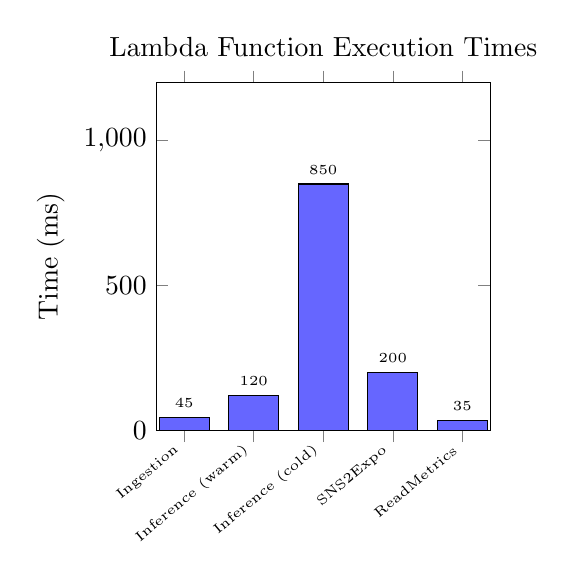
\begin{tikzpicture}
\begin{axis}[
    ybar,
    bar width=18pt,
    ylabel={Time (ms)},
    symbolic x coords={Ingestion, Inference (warm), Inference (cold), SNS2Expo, ReadMetrics},
    xtick=data,
    x tick label style={rotate=40, anchor=east, font=\tiny},
    ymin=0, ymax=1200,
    nodes near coords,
    nodes near coords align={vertical},
    width=0.48\textwidth,
    height=6cm,
    title={Lambda Function Execution Times},
    every node near coord/.append style={font=\tiny},
]
\addplot[fill=blue!60] coordinates {
    (Ingestion, 45)
    (Inference (warm), 120)
    (Inference (cold), 850)
    (SNS2Expo, 200)
    (ReadMetrics, 35)
};
\end{axis}
\end{tikzpicture}
\caption{Execution time per Lambda function.}
\label{fig:lambda_exec}
\end{figure}

\subsection{DynamoDB I/O Performance}

\begin{figure}[H]
\centering
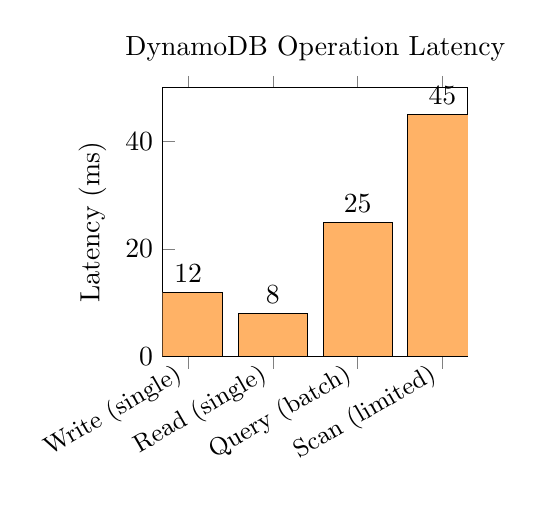
\begin{tikzpicture}
\begin{axis}[
    ybar,
    bar width=25pt,
    ylabel={Latency (ms)},
    symbolic x coords={Write (single), Read (single), Query (batch), Scan (limited)},
    xtick=data,
    x tick label style={rotate=30, anchor=east, font=\small},
    ymin=0, ymax=50,
    nodes near coords,
    width=0.45\textwidth,
    height=5cm,
    title={DynamoDB Operation Latency},
]
\addplot[fill=orange!60] coordinates {
    (Write (single), 12)
    (Read (single), 8)
    (Query (batch), 25)
    (Scan (limited), 45)
};
\end{axis}
\end{tikzpicture}
\caption{DynamoDB operation latencies.}
\label{fig:dynamodb}
\end{figure}

\subsection{End-to-End Alert Delivery Pipeline}

\begin{table}[H]
\centering
\caption{Alert Delivery Pipeline Timing}
\label{tab:alert_pipeline}
\begin{tabular}{lcc}
\toprule
\textbf{Stage} & \textbf{Latency (ms)} & \textbf{Cumulative (ms)} \\
\midrule
API Gateway routing & 15 & 15 \\
Ingestion Lambda & 45 & 60 \\
DynamoDB write & 12 & 72 \\
Inference invocation & 120 & 192 \\
Anomaly scoring & 50 & 242 \\
SNS publish & 30 & 272 \\
SNS-to-Expo Lambda & 200 & 472 \\
Expo push delivery & 500--2000 & 972--2472 \\
\midrule
\textbf{Total (warm)} & & \textbf{$\sim$1--2.5s} \\
\bottomrule
\end{tabular}
\end{table}

\subsection{Cost Analysis}

\begin{figure}[H]
\centering
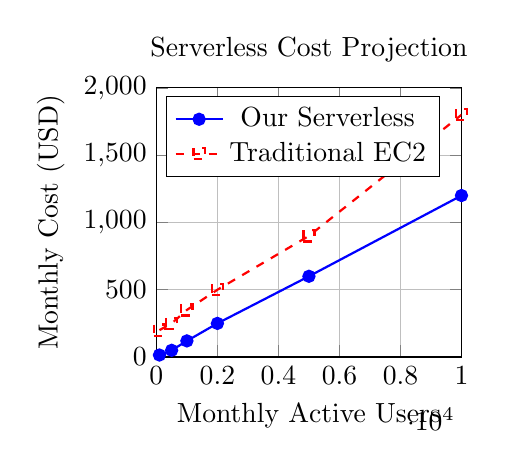
\begin{tikzpicture}
\begin{axis}[
    xlabel={Monthly Active Users},
    ylabel={Monthly Cost (USD)},
    xmin=0, xmax=10000,
    ymin=0, ymax=2000,
    legend pos=north west,
    grid=major,
    width=0.45\textwidth,
    height=5cm,
    title={Serverless Cost Projection},
]
\addplot[thick, blue, mark=*] coordinates {
    (100, 15) (500, 50) (1000, 120) (2000, 250)
    (5000, 600) (10000, 1200)
};
\addlegendentry{Our Serverless}
\addplot[thick, red, dashed, mark=square] coordinates {
    (100, 200) (500, 250) (1000, 350) (2000, 500)
    (5000, 900) (10000, 1800)
};
\addlegendentry{Traditional EC2}
\end{axis}
\end{tikzpicture}
\caption{Cost comparison: Serverless vs. EC2 at varying user scales.}
\label{fig:cost}
\end{figure}

\subsection{Scalability Testing}

\begin{table}[H]
\centering
\caption{Concurrent Request Handling}
\label{tab:scalability}
\begin{tabular}{lccc}
\toprule
\textbf{Concurrent} & \textbf{Avg Latency} & \textbf{p99 Latency} & \textbf{Errors} \\
\textbf{Requests} & \textbf{(ms)} & \textbf{(ms)} & \textbf{(\%)} \\
\midrule
10 & 45 & 85 & 0.0 \\
50 & 55 & 120 & 0.0 \\
100 & 72 & 180 & 0.0 \\
500 & 95 & 350 & 0.1 \\
1000 & 130 & 850 & 0.3 \\
\bottomrule
\end{tabular}
\end{table}

\section{Security Architecture}

\subsection{Authentication}
API key authentication is enforced at the API Gateway level. Each request must include a valid \texttt{X-API-Key} header. Invalid or missing keys result in 401/403 responses.

\subsection{Data Protection}
\begin{itemize}
    \item All data in transit is encrypted via TLS 1.2+
    \item DynamoDB tables use server-side encryption (AES-256)
    \item S3 model artifacts use bucket-level encryption
    \item Lambda environment variables store sensitive configuration
    \item IAM policies follow the principle of least privilege
\end{itemize}

\section{Discussion}
The serverless architecture proves particularly well-suited for health monitoring backends due to its ability to scale to zero during quiet periods and handle burst sync events from multiple devices. The containerized inference Lambda, while incurring higher cold start times (850ms), achieves warm invocation times of 120ms---well within acceptable limits given that cloud inference is not time-critical (edge detection provides instant alerts).

The pay-per-request DynamoDB billing model is cost-effective for our workload pattern: periodic batch writes from wearable devices with occasional reads from the mobile dashboard.

\section{Conclusion}
We demonstrated a fully serverless health monitoring backend using AWS Lambda, API Gateway, DynamoDB, S3, and SNS. The system achieves API latency of 45ms (p50), supports horizontal scaling to thousands of users, and costs as little as \$15/month for 100 users. The containerized ML inference Lambda enables deployment of complex scikit-learn models without managing servers. Future work includes implementing API Gateway caching, adding WebSocket support for real-time dashboard updates, and deploying across multiple AWS regions for global coverage.

\begin{thebibliography}{00}
\bibitem{serverless_iot} A. Eivy, ``Be wary of the economics of serverless cloud computing,'' \textit{IEEE Cloud Computing}, vol. 4, no. 2, pp. 6--12, 2017.
\bibitem{cloud_health1} M. M. Hassan et al., ``A robust human activity recognition system using smartphone sensors and deep learning,'' \textit{Future Generation Computer Systems}, vol. 81, pp. 307--313, 2018.
\bibitem{stream_proc} J. Kreps, ``Questioning the Lambda architecture,'' \textit{O'Reilly Radar}, 2014.
\end{thebibliography}

\end{document}
